
\noindent This chapter covers the following ideas. (These are subject to change, as I write the notes.)

\begin{enumerate}

\item Find the currents in electrical systems involving batteries and resistors, using both Gaussian elimination and Cramer's rule.
\item Find interpolating polynomials. Use the transpose and inverse of a matrix to solve the least squares regression problem of fitting a line to a set of data.
\item Find the partial fraction decomposition of a rational function. Utilize this decomposition to integrate rational functions.
\item Describe a Markov process. Explain how an eigenvector of the eigenvalue $\lambda=1$ is related to the limit of powers of the transition matrix.
\item Explain how to generalize the derivative to a matrix. Use this generalization to locate optimal values of the function using the second derivative test. Explain the role  of eigenvalues and eigenvectors in the second derivative test.
\end{enumerate}

{\Huge The order of the following problems is not set.  Feel free to work on them, but realize that the order may change as I continue writing over the weekend.}

\section{Vector Fields}
In multivariate calculus, we studied vector fields of the form $\vec F(x,y) = (M,N)$, where $M$ and $N$ are functions of $x$ and $y$.  If you compute the derivative of a vector field, you obtain the square matrix
$$D\vec F(x,y) =
\begin{bmatrix}
\partial M/\partial x &
\partial M/\partial y \\
\partial N/\partial x &
\partial N/\partial y 
\end{bmatrix}.
$$ 
The eigenvalues and eigenvectors of this matrix provide us with a wealth of information about the vector field.  The next few problems have you discover many of these key ideas.  We'll return to these problems throughout the semester, especially when we start studying systems of differential equations.

\begin{problem}
Consider the vector field $\vec F(x,y) = (2x+y, x+2y)$. 
\begin{enumerate}
 \item At each of the 8 points given by $(\pm 1, \pm 1)$, $(0, \pm 1)$, $(\pm 1, 0)$, sketch the vector $\vec F(x,y)$ with it's base at the input point (so at point $(1,0)$, sketch $(2,1)$, a vector starting at $(1,0)$ and ending at $(3,1)$).  This provides us with a rough sketch of the vector field.
 \item Compute $A=D\vec F(x,y)$. It should be a 2 by 2 matrix. 
 \item Remember that we say a vector $\vec x$ is an eigenvector if $A\vec x = \lambda \vec x$.  For any of the vectors from part 1., did you find that $A\vec x = \lambda \vec x$?  Which ones (these are eigenvectors)?  By how much was the vector $\vec x$ stretched (these are eigenvalues)? 
 \item Now compute the eigenvalues and eigenvectors of this matrix, using the algorithm from the previous chapter.  You should obtain the same answer as part 3.
\end{enumerate}
\end{problem}
The problem above had two positive eigenvalues. In the next problem, your goal is to determine what a vector field looks like when you have a positive eigenvalues, and a negative eigenvalue.

\begin{problem}
Complete the following:
\begin{enumerate}
 \item For the vector field $\vec F = (x, 2x-y)$, compute the eigenvalues and eigenvectors of $D\vec F(x,y)$. 
 \item For the vector field $\vec F = (x-4y, -6x-y)$, compute the eigenvalues and eigenvectors of $D\vec F(x,y)$. 
 \item With each vector field, use a computer to construct a vector field plot.  In the plot, please show us how to see the eigenvectors, together with which which eigenvector corresponds to a positive eigenvalues, and which corresponds to a negative eigenvalue. You can construct vector fields in Wolfram|Alpha by typing ``vector field plot'' in the input box, or just  follow the link \url{http://www.wolframalpha.com/input/?i=vector+field+plot&lk=4&num=2}.
 \item Add to your plots several trajectories, i.e. a path that a particle would follow if $\vec F$ represents the tangent vectors of the path.  Think, ``If I dropped a really light particle in this field, representing water current, where would the particle go? \note{adding an example here could help them, that way they know what they are doing.  A link to an appropriate vector field plot would do it.}
\end{enumerate}
\end{problem}

\begin{problem}
The following three vector fields have imaginary eigenvalues. Compute the eigenvalues for each, construct a vector field plot, and on the plot add several trajectories (the path followed by a particle that is dropped into this field).
\begin{enumerate}
 \item $\vec F = (-2y,x)$. 
 \item $\vec F = (-x+y, -x-y)$.
 \item $\vec F = (x-y, x)$ 
\end{enumerate}
Make a conjecture as to why one spirals in, one spirals out, and one just wraps around in ellipses. We'll address this conjecture in class.
\end{problem}

The next problem requires that you are on a computer that can use Mathematica. These computers are available in the Ricks, Austin, Romney, and library.  Alternately, you can download VMWare that will allow you to use Mathematica for free from your computer, provided you head to \url{https://vdiview.byui.edu/}. You can download step-by-step instructions from \url{http://www.byui.edu/help-desk/categories/vdivmware}. Please take a moment and make sure you can access Mathematica.

\begin{problem}
Start by downloading the Mathematica notebook VectorFields.nb.  The goal of this problem is to make a connection between a vector field and it's corresponding eigenvalues/eigenvectors. Once the notebook is open, click somewhere in the text, hold down Shift, and then press Enter.  This will evaluate the commands and produce a vector field plot. You can click on the bubbles with crosshairs in them to adjust the vectors (which are the columns of the matrix).
 \begin{enumerate}
  \item If the vector field pushes things outwards in all directions, what do you know about the eigenvalues?
  \item How can you tell, by looking at a vector field plot, that one eigenvalue is positive, and the other is negative?
  \item If the vector field spirals outwards, what do you know about the eigenvalues?
  \item If the vector field pulls everything inwards, what do you know about the eigenvalues?
  \item If the vector field spirals inwards, what do you know about the eigenvalues?
  \item What happens when you have a repeated eigenvalue? (This one has lots of correct answers, and it a topic for much further discussion in chapter 10.)
 \end{enumerate}
\end{problem}



\subsection{Second Derivative Test}

Have them compute the first and second derivative (call it the Hessian), and then have them compute the eigenvalues and eigenvectors of the Hessian.  Have them draw this vector field  as above (as an approximation to the gradient).  Then ask them to state if you have a max or min.  They should be able to tell the conditions under which you get a maximum by just asking about gradients.  Have them do 3 problems like this, with the last having multiple critical values, maybe the last 2. 

Let's start with a review from first semester calculus. If a function $y=f(x)$ has a relative extremum at $x=c$, then $f^\prime(c)=0$ or the derivative is undefined. The places where the derivative is either zero or undefined are called critical values of the function. The first derivative test allows you to check the value of the derivative on both sides of the critical value and then interpret whether that point is a maximum or minimum using increasing/decreasing arguments.  The second derivative test requires you to compute the second derivative at $x=c$. If $f^{\prime\prime}(c)>0$ (the function is concave upwards), then the function has a minimum at $x=c$. If $f^{\prime\prime}(c)<0$ (the function is concave downwards), then the function has a maximum at $x=c$. If $f^{\prime\prime}(c)=0$, then the second derivative test fails. 

\begin{example}
The function $f(x) = x^3-3x$ has derivatives $f^\prime = 3x^2-3$ and $f^{\prime\prime}=6x$.  The first derivative is zero when $3(x^2-1)=3(x-1)(x+1)=0$, or $x=\pm 1$.  The second derivative at $x=1$ is $6$ (concave upwards), so there is a minimum at $x=1$.  The second derivative at $x=-1$ is $-6$ (concave downwards), so there is a maximum at that point. 
\end{example}

We're now ready to extend this idea to all functions of the form $f:{\mathbb{R}}^n\to{\mathbb{R}}$ (the output is 1 dimensional, so that it makes sense to talk about a largest or smallest number). We will only consider the case $n=2$, as it simplifies the computations and provides all that is needed to extend to all dimensions. The first derivative test breaks down in every dimension past the first, because there are more than 2 ways to approach a point of the domain (you can't just look at the left side or right side). However, at a local extremum, the derivative is still zero, which often results in solving a system of equations. In higher dimensions, there are three classifications of critical points: maximum, minimum, or saddle point (a point where the tangent plane is horizontal, but in some directions you increase and in other directions you decrease). 

The second derivative test does not break down. Consider the function $z=f(x,y)$. Its derivative $Df(x,y) = \begin{bmatrix}f_x&f_y\end{bmatrix}$ is a function with two inputs and two outputs. The second derivative {$D^2f (x,y)= \begin{bmatrix}f_{xx}&f_{xy}\\f_{yx}&f_{yy}\end{bmatrix} $} is a {$2\times 2$} square matrix called the Hessian of $f$. This matrix will always be symmetric, in that the transpose of the matrix equals itself (because $f_{xy}=f_{yx}$).  At a critical point (where the first derivative is zero), the eigenvalues of $D^2f$ give the directional second derivative in the direction of a corresponding eigenvector. The largest eigenvalue is the largest possible value of the second derivative in any direction and the smallest eigenvalue is the smallest possible value of the second derivative in any direction. 

The \textbf{second derivative test} \marginpar{the second derivative test with eigenvalues} is the following. Start by finding all the critical points (places where the derivative is zero). Then find the eigenvalues of the second derivative. Each eigenvalue represents the 2nd directional derivative in the direction of a corresponding eigenvector. In every other direction, the directional 2nd derivative is between the smallest and largest eigenvalue.  
\begin{enumerate}
	\item If the eigenvalues are all positive at a critical point, then in every direction the function is concave upwards. The function has a minimum at that critical point.
	\item If the eigenvalues are all negative at a critical point, then in every direction the function is concave downwards. The function has a maximum there.
	\item If there is a positive eigenvalue and a negative eigenvalue, the function has a saddle point there.  
	\item If either the largest or smallest eigenvalue is zero, then the second derivative test fails. 
\end{enumerate}
Eigenvalues are the key numbers needed to generalize optimization to all dimensions. A proof of this fact is beyond the scope of this class. 

\begin{example}
For the function {$f(x,y)=x^2+xy+y^2$}, the gradient is $Df = \begin{bmatrix}2x+y&x+2y \end{bmatrix}$, which is zero only at $x=0,y=0$ (solve the system of equations $2x+y=0,x+2y=0$). The Hessian is $D^2f = \begin{bmatrix}2&1 \\1&2\end{bmatrix}$. The eigenvalues are found by solving $0=\det \begin{bmatrix}2-\lambda &1 \\1&2-\lambda \end{bmatrix} = (2-\lambda)^2-1 = 4-4\lambda+\lambda^2 -1 = (\lambda-3)(\lambda-1)$, so $\lambda = 3,1$ are the eigenvalues.  Since both eigenvalues are positive, the function is concave upwards in all directions, so there is a minimum at $(0,0)$.  

The eigenvectors of the Hessian help us understand more about the graph of the function.  An eigenvector corresponding to 3 is (1,1), and corresponding to 1 is (-1,1). These vectors are drawn in figure \ref{2ndder}, together with two parabolas whose 2nd derivatives are precisely 3 and 1.  The parabola which opens upwards the most quickly has a 2nd derivative of 3.  The other parabola has a second derivative of 1. In every other direction, the 2nd derivative would be between 1 and 3.

\end{example}

%\marginpar{{
\begin{figure}[ht
]\begin{center}
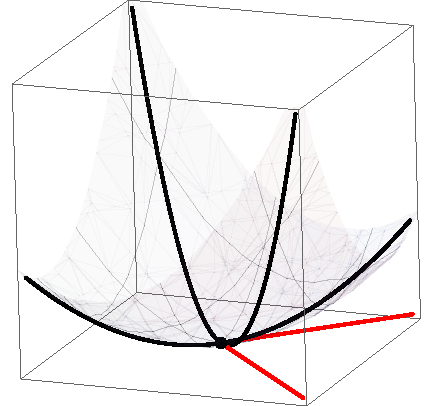
\includegraphics[width=2in]{support/2nddertest1}
\hspace{.5in}
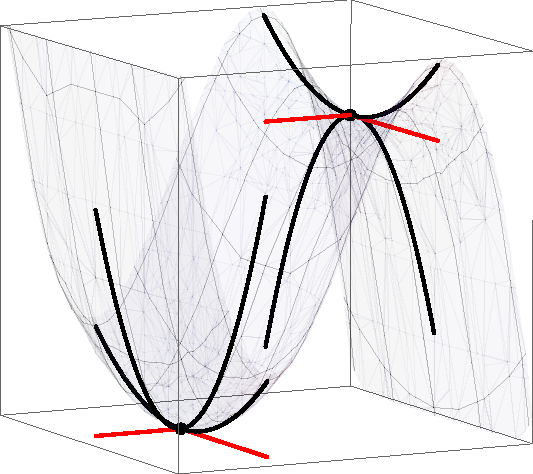
\includegraphics[width=2in]{support/2nddertest2}
\end{center}
\caption{The eigenvectors of the second derivative tell you the directions in which the 2nd derivative is largest and smallest. At each critical point, two eigenvectors are drawn as well as a parabola whose second derivative (the eigenvalue) matches the second derivative of the surface in the corresponding eigenvector direction.}
\label{2ndder}
\end{figure}
%}}


\begin{example}
For the function {$f(x,y)=x^3-3x+y^2-4y$}, the gradient is $Df = \begin{bmatrix}3x^2-3&2y-4 \end{bmatrix}$, which is zero at $x=1,y=2$ or $x=-1,y=2$. Hence there are two critical points, so we have to find two sets of eigenvalues. The Hessian is $D^2f = \begin{bmatrix}6x&0 \\0&2\end{bmatrix}$. When $x=-1,y=2$, the eigenvalues of $\begin{bmatrix}-6&0 \\0&2\end{bmatrix}$ are $\lambda=-6,2$. Since one is positive and one is negative, there is a saddle point at $(-1,2)$. When $x=1,y=2$, the eigenvalues of $\begin{bmatrix}6&0 \\0&2\end{bmatrix}$ are $\lambda=6,2$. Since both are positive, there is a minimum at $(-1,2)$ (as in every direction the function is concave upwards).

Again the eigenvectors help us understand how the function behaves, as illustrated in figure \ref{2ndder}.  At (1,2) we have an eigenvector (1,0) corresponding to 6, and (0,1) corresponding to 2. In both eigenvector directions the function is concave upwards, but opens more stepply in the (1,0) direction as 6 is bigger than 2.  At (-1,2) the we have an eigenvector (1,0) corresponding to -6, and (0,1) corresponding to 2. The functions opens stepply downwards in the (1,0) direction, and upwards in the (0,1) direction. 
\end{example}








\subsection{Systems of Differential Equations}
Introduce the language of systems of differential equations.  Then have them solve graphically a system by drawing the trajectories in the phase plane (it's the exact same as the vector field section, with no change).  I could pull in a mutalism (bees and plants) or a competitive hunter, or an (xxxxxx done arms race example).  All of which are great, but add more to the learning.  This could be a really good section.  

I could also introduce tank mixing (a conservation problem, to tie the two together, this is perfect right here at the end).  The tank mixing problem connects the conservation part to the eigenvalues part.  We wouldn't have a complete solution to the problem, but we could approximate the solution. After doing tank mixing, you should mention the huge applications, and how this is basically a flow problem (so relate to flux and divergence).  Economic import/export.  Immigration. Spread of Disease. Spreading of noxious weeds and more.  This is a huge idea that we should start soon.




\section{Conservation Laws}
Many problems in nature arise from conservation laws.  These laws generally focus on the principle that matter is neither is created nor destroyed, rather it is just moved, changed, or something.  Any of the following could be viewed as a conservation law:
\begin{itemize}
 \item What comes in must come out.
 \item Voltage supplied equals voltage suppressed.
 \item Atoms before equal atoms after.
 \item The change in a quantity is how much it increases minus how much it decreases.
 \item Current in equals current out.
\end{itemize}
The following problems related to some conservation law.  You'll see similar laws in your future classes, regardless of your discipline.

\subsection{Network Flow}
Imagine that

\begin{problem}
Have them set up a system of cars at specific intersections.  Give them the inflows at some, and the outflows at others.  Then ask them how many cars are on each road at any given time. 
\end{problem}

\begin{problem}
 Use the same system as the previous, but now close one of the roads.  Then ask them to solve the problem again.  They are predicting what will happen to traffic patterns if you close down a road.
\end{problem}
Connect this to network traffic on the internet, airplane routes, and more.

\subsection{Markov Processes}
Introduce the car rental company problem.  The conservation law states....  Then have them set up a system
\begin{problem}
 Have them setup a matrix equation. We wish to solve the problem...  If this has a solution, then what is the corresponding eigenvalue of the coefficient matrix.  Solve for the eigenvector.
\end{problem}

\begin{problem}
Do the land problem (residential, commercial, economic). 
\end{problem}


\begin{problem}
 Use Larry's problem.  This connects to value of commodities.
\end{problem}


Matrices can be used to model a process called a Markov Process. To fit this kind of model, a process must have specific states, and the matrix which models the process is a transition matrix which specifies how each state will change through a given transition. An example of a set of states is ``open'' or ``closed'' in an electrical circuit, or ``working properly'' and ``working improperly'' for operation of machinery at a manufacturing facility. A car rental company which rents vehicles in different locations can use a Markov Process to keep track of where their inventory of cars will be in the future. Stock market analysts use Markov processes and a generalization called stochastic processes to make predictions about future stock values.

\begin{example} Let's illustrate a Markov Process related to classifying land in some region as ``Residential,'' ``Commercial,'' or ``Industrial.'' Suppose in a given region over a 5 year time span that 80\% of residential land will remain residential, 10\% becomes commercial, and 10\%  becomes industrial.  For commerical land, 70\% remains commercial, 20\% becomes residential, and 10\% becomes industrial.  For industrial land, 70\% remains industrial, 30\% becomes commercial, and 0\% becomes residential.  To find what happens at the end of a 5 year period, provided we know the current $R$, $C$, and $I$ values, we could just compute 
$$
\begin{array}{rl}
R_{\text{new}} &= .8 R+ .2 C+0 I\\ 
C_{\text{new}} &= .1 R+ .7 C+.3 I\\ 
I_{\text{new}} &= .1 R+ .1 C+.7 I 
\end{array}
\xrightarrow{\text{matrix form}}
\begin{bmatrix}
R_{\text{new}}\\ 
C_{\text{new}}\\ 
I_{\text{new}} 
\end{bmatrix}
=
\begin{bmatrix}
.8& .2 &0 \\ 
.1& .7 &.3\\ 
.1& .1 &.7 
\end{bmatrix}
\begin{bmatrix}
R\\ 
C\\ 
I 
\end{bmatrix}
$$
The matrix on the right above is called the transition matrix of the Markov process. 
\marginpar{
$ \begin{array}{rl}
&\begin{array}{ccc} R&C&I \end{array} \\
 \begin{array}{c} \text{to }R\\ \text{to }C\\ \text{to }I \end{array}& 
\begin {bmatrix}  .8&.2&0\\.1&.7&.3\\.1&.1&.7 \end {bmatrix} \\
\multicolumn{2}{c}{\text{Transition Matrix}}
\end{array}
$} 
It is a matrix where each column relates to one of the ``states,'' and the numbers in that column are the proportions of the column state that will change to the row state through the transition (the ordering on row and column states is the same). 
We calculate the next ``state'' by multiplying our current state by the transition matrix. If current land use is about 50\% residential, 30\% commercial, and 20\% industrial, then 5 years later the land use would be 
$$ 
 \begin {bmatrix} .8&.2&0\\.1&.7&.3\\.1&.1&.7 \end {bmatrix}
 \begin {bmatrix} 50\\30\\20 \end {bmatrix}
 =   \begin {bmatrix} 46\\ 32 \\ 22\end {bmatrix}
$$  If the same transitions in land use continue, we can multiply the previous projection (state) by the transition matrix to obtain a 10 and 15 year projection for land use:  
\begin{center}\begin{tabular}{cc}
$
\begin {bmatrix} .8&.2&0\\.1&.7&.3\\.1&.1&.7 \end {bmatrix}
\begin {bmatrix} 46\\ 32 \\ 22 \end {bmatrix}
 =   \begin {bmatrix} 43.2\\ 33.6 \\ 23.2\end {bmatrix}
$ 
&
$
\begin {bmatrix} .8&.2&0\\.1&.7&.3\\.1&.1&.7 \end {bmatrix}
\begin {bmatrix} 43.2\\ 33.6 \\ 23.2 \end {bmatrix}
 =   \begin {bmatrix} 41.28\\ 34.8\\ 23.92\end {bmatrix}
$ 
\\
10 Year Projection 
&15 Year Projection 
\end{tabular}\end{center}
As we continue to multiply on the left by our transition matrix, each time we add 5 more years to our projection. This projection is valid as long as the same trends continue. 
\end{example}









%\subsection{Steady State Solutions}


Consider the land use example from above.  Let $\vec x_0$ be our initial state. If our transition matrix $A$ remains the same forever, what will eventually happen to the proportion of land devoted to residential, commercial, or industrial use? We can write each new state as powers of the transition matrix $A$ by writing 
$\vec x_{1} = A \vec x_{0}$, $\vec x_{2}=A \vec x_{1} = AA\vec x_{0} = A^2\vec x_{0}$, $\vec x_{3}= A^3\vec x_{0}$, and $\vec x_{n}= A^n\vec x_{0}$.  What happens to the product $A^n\vec x_0$ as $n\to \infty$? Can we reach a state $\vec x = (R,C,I)$ such that $A \vec x=\vec x$, the next state is the same as the current? If this occurs, then any future transitions will not change the state either. This state $\vec x$ is called a steady state, since it does not change when multiplied by the transition matrix (it remains steady). 

Finding a steady state is an eigenvalue-eigenvector problem, as we are looking for a solution to the equation $A\vec x = 1\vec x$ (where the eigenvalue is 1). For any Markov process (where the columns of the matrix sum to 1), the number 1 will always be an eigenvalue. All we have to do is find the eigenvectors corresponding to the eigenvalue 1. The solution to the problem $\ds\lim_{n\to\infty}A^n \vec x_0$ is this steady state, and is an eigenvector. For the land use Markov process, an eigenvector (using technology) corresponding to 1 is $\begin{bmatrix}\frac{3}{2}&\frac32&1\end{bmatrix}^T$. Since any multiple of an eigenvector is again an eigenvector, we can multiply by a constant so that the proportions sum to 100. Multiplying by 2  we have $\begin{bmatrix}3&3&2\end{bmatrix}^T$, which means that the ratio of land will be 3 acres residential to 3 acres commercial to 2 acres industrial. To write this in terms of percentages, divide each component by 8 (the sum $3+3+2$) to obtain $3/8:3/8:2/8$ or multiplying by 100 we have $37.5\%:37.5\%:25\%$. These are the long term percentages of land use.

More examples are available in the handwritten solutions to problems, available online.














\subsection{Kirchoff's Electrical Laws}
Gustav Kirchoff discovered two laws of electricity that pertain to the conservation of charge and energy.  To describe these laws, we must first discuss voltage, resistance, and current.  Current is the flow of electricity, and often it can be compared to the flow of water.  As a current passes across a conductor, it encounters resistance. Ohm's law states that the product of the resistance $R$ and current $I$ across a conductor equals the voltage $V$, i.e. $RI=V$. If the voltage remains constant, then a large resistance corresponds to a small current. A resistor is an object with high resistance which is placed in an electrical system to slow down the flow (current) of electricity.  Resistors are measured in terms of ohms, and the larger the ohms, the smaller the current.  Figure \ref{ecir} illustrates two introductory electrical systems. 


\begin{figure}[htb]
\begin{center}
\begin{tabular}{cc}
\renewcommand{\myscale}{.3}
\begin{tikzpicture}[scale=\myscale,inner sep=1pt]
%\draw[help lines,step=1cm] (0,0) grid (12,6);

%Source - like a battery
\node[label=right:$E$] at (0,3)
{{\begin{tikzpicture}[scale=\myscale]
%	\useasboundingbox (-.5,-3) rectangle (.5,3);
	\draw (0,0) circle (1cm);
	\draw (.3,.5) -- (-.3,.5);
	\draw (0,.2) -- (0,.8);
	\draw (.3,-.5) -- (-.3,-.5);
	\draw (0,1) -- (0,3);
	\draw (0,-1) -- (0,-3);
	\end{tikzpicture}
}};

%Resistor
\node[label=right:$R_2$] at (6,3) 
{{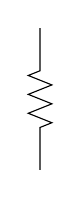
\begin{tikzpicture}[scale=\myscale]
%	\useasboundingbox (0,-3) rectangle (0,3);
	\draw (0,-3) -- ++(0,1.8) -- ++(.5,.2) 
		-- ++(-1,.4) -- ++(1,.4)
		-- ++(-1,.4) -- ++(1,.4)
		-- ++(-1,.4) -- ++(.5,.2)
		-- ++(0,1.8) ;
	\end{tikzpicture}
}};

%Resistor
\node[label=above:$R_1$] at (3,0) 
{{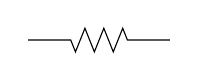
\begin{tikzpicture}[scale=\myscale,rotate=90]
%	\useasboundingbox (0,-3) rectangle (0,3);
	\draw (0,-3) -- ++(0,1.8) -- ++(.5,.2) 
		-- ++(-1,.4) -- ++(1,.4)
		-- ++(-1,.4) -- ++(1,.4)
		-- ++(-1,.4) -- ++(.5,.2)
		-- ++(0,1.8) ;
	\end{tikzpicture}
}};

%Resistor
\node[label=right:$R_3$] at (12,3) 
{{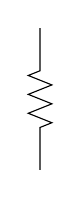
\begin{tikzpicture}[scale=\myscale,rotate=0]
%	\useasboundingbox (0,-3) rectangle (0,3);
	\draw (0,-3) -- ++(0,1.8) -- ++(.5,.2) 
		-- ++(-1,.4) -- ++(1,.4)
		-- ++(-1,.4) -- ++(1,.4)
		-- ++(-1,.4) -- ++(.5,.2)
		-- ++(0,1.8) ;
	\end{tikzpicture}
}};

%Straight Path
\node at (3,6) 
{{\begin{tikzpicture}[scale=\myscale,rotate=90]
	\draw (0,-3) -- (0,3);
	\end{tikzpicture}
}};

%Straight Path
\node at (9,6) 
{{\begin{tikzpicture}[scale=\myscale,rotate=90]
	\draw (0,-3) -- (0,3);
	\end{tikzpicture}
}};

%Straight Path
\node at (9,0) 
{{\begin{tikzpicture}[scale=\myscale,rotate=90]
	\draw (0,-3) -- (0,3);
	\end{tikzpicture}
}};


%Arrow to represent Current
\node[label=above:$i_1$] at (3,6) 
{{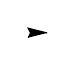
\begin{tikzpicture}[scale=\myscale,rotate=-90]
%	\useasboundingbox (0,-.4) rectangle (0,.4);
	\filldraw (0,.4) -- (-.2,-.4) -- (0,-.3) -- (.2,-.4);
	\end{tikzpicture}
}};

%Arrow to represent Current
\node[label=right:$i_2$] at (6,5) 
{{
\begin{tikzpicture}[scale=\myscale,rotate=180]
%	\useasboundingbox (0,-.4) rectangle (0,.4);
	\filldraw (0,.4) -- (-.2,-.4) -- (0,-.3) -- (.2,-.4);
	\end{tikzpicture}
}};

%Arrow to represent Current
\node[label=above:$i_3$] at (9,6) 
{{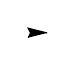
\begin{tikzpicture}[scale=\myscale,rotate=-90]
%	\useasboundingbox (0,-.4) rectangle (0,.4);
	\filldraw (0,.4) -- (-.2,-.4) -- (0,-.3) -- (.2,-.4);
	\end{tikzpicture}
}};

%Node
\node at (6,6) 
{{\begin{tikzpicture}[scale=\myscale,rotate=-90]
%	\useasboundingbox (0,-.4) rectangle (0,.4);
	\filldraw (0,0) circle (.15cm);
	\end{tikzpicture}
}};

%Node
\node at (6,0) 
{{\begin{tikzpicture}[scale=\myscale,rotate=-90]
%	\useasboundingbox (0,-.4) rectangle (0,.4);
	\filldraw (0,0) circle (.15cm);
	\end{tikzpicture}
}};

\end{tikzpicture}

&
\renewcommand{\myscale}{.3}
\begin{tikzpicture}[scale=\myscale,inner sep=1pt]
%\draw[help lines,step=1cm] (0,0) grid (18,6);

%Source - like a battery
\node[label=right:$E$] at (0,3) 
{{\begin{tikzpicture}[scale=\myscale]
%	\useasboundingbox (-.5,-3) rectangle (.5,3);
	\draw (0,0) circle (1cm);
	\draw (.3,.5) -- (-.3,.5);
	\draw (0,.2) -- (0,.8);
	\draw (.3,-.5) -- (-.3,-.5);
	\draw (0,1) -- (0,3);
	\draw (0,-1) -- (0,-3);
	\end{tikzpicture}
}};

%Resistor
\node[label=right:$R_2$] at (6,3) 
{{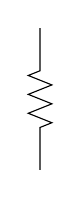
\begin{tikzpicture}[scale=\myscale]
%	\useasboundingbox (0,-3) rectangle (0,3);
	\draw (0,-3) -- ++(0,1.8) -- ++(.5,.2) 
		-- ++(-1,.4) -- ++(1,.4)
		-- ++(-1,.4) -- ++(1,.4)
		-- ++(-1,.4) -- ++(.5,.2)
		-- ++(0,1.8) ;
	\end{tikzpicture}
}};

%Resistor
\node[label=above:$R_1$] at (3,0) 
{{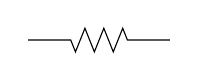
\begin{tikzpicture}[scale=\myscale,rotate=90]
%	\useasboundingbox (0,-3) rectangle (0,3);
	\draw (0,-3) -- ++(0,1.8) -- ++(.5,.2) 
		-- ++(-1,.4) -- ++(1,.4)
		-- ++(-1,.4) -- ++(1,.4)
		-- ++(-1,.4) -- ++(.5,.2)
		-- ++(0,1.8) ;
	\end{tikzpicture}
}};

%Resistor
\node[label=above:$R_3$] at (9,6) 
{{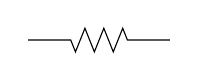
\begin{tikzpicture}[scale=\myscale,rotate=90]
%	\useasboundingbox (0,-3) rectangle (0,3);
	\draw (0,-3) -- ++(0,1.8) -- ++(.5,.2) 
		-- ++(-1,.4) -- ++(1,.4)
		-- ++(-1,.4) -- ++(1,.4)
		-- ++(-1,.4) -- ++(.5,.2)
		-- ++(0,1.8) ;
	\end{tikzpicture}
}};

%Resistor
\node[label=right:$R_4$] at (12,3) 
{{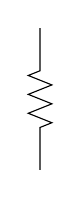
\begin{tikzpicture}[scale=\myscale,rotate=0]
%	\useasboundingbox (0,-3) rectangle (0,3);
	\draw (0,-3) -- ++(0,1.8) -- ++(.5,.2) 
		-- ++(-1,.4) -- ++(1,.4)
		-- ++(-1,.4) -- ++(1,.4)
		-- ++(-1,.4) -- ++(.5,.2)
		-- ++(0,1.8) ;
	\end{tikzpicture}
}};

%Resistor
\node[label=right:$R_5$] at (18,3) 
{{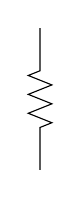
\begin{tikzpicture}[scale=\myscale,rotate=0]
%	\useasboundingbox (0,-3) rectangle (0,3);
	\draw (0,-3) -- ++(0,1.8) -- ++(.5,.2) 
		-- ++(-1,.4) -- ++(1,.4)
		-- ++(-1,.4) -- ++(1,.4)
		-- ++(-1,.4) -- ++(.5,.2)
		-- ++(0,1.8) ;
	\end{tikzpicture}
}};

%Resistor
\node[label=above:$R_6$] at (9,0) 
{{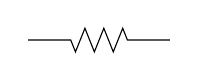
\begin{tikzpicture}[scale=\myscale,rotate=90]
%	\useasboundingbox (0,-3) rectangle (0,3);
	\draw (0,-3) -- ++(0,1.8) -- ++(.5,.2) 
		-- ++(-1,.4) -- ++(1,.4)
		-- ++(-1,.4) -- ++(1,.4)
		-- ++(-1,.4) -- ++(.5,.2)
		-- ++(0,1.8) ;
	\end{tikzpicture}
}};









%Straight Path
\node at (3,6) 
{{\begin{tikzpicture}[scale=\myscale,rotate=90]
	\draw (0,-3) -- (0,3);
	\end{tikzpicture}
}};

%Straight Path
\node at (15,6) 
{{\begin{tikzpicture}[scale=\myscale,rotate=90]
	\draw (0,-3) -- (0,3);
	\end{tikzpicture}
}};

%Straight Path
\node at (15,0) 
{{\begin{tikzpicture}[scale=\myscale,rotate=90]
	\draw (0,-3) -- (0,3);
	\end{tikzpicture}
}};






%Arrow to represent Current
\node[label=above:$i_1$] at (3,6) 
{{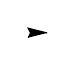
\begin{tikzpicture}[scale=\myscale,rotate=-90]
%	\useasboundingbox (0,-.4) rectangle (0,.4);
	\filldraw (0,.4) -- (-.2,-.4) -- (0,-.3) -- (.2,-.4);
	\end{tikzpicture}
}};

%Arrow to represent Current
\node[label=right:$i_2$] at (6,5) 
{{
\begin{tikzpicture}[scale=\myscale,rotate=180]
%	\useasboundingbox (0,-.4) rectangle (0,.4);
	\filldraw (0,.4) -- (-.2,-.4) -- (0,-.3) -- (.2,-.4);
	\end{tikzpicture}
}};

%Arrow to represent Current
\node[label=above:$i_3$] at (7,6) 
{{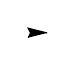
\begin{tikzpicture}[scale=\myscale,rotate=-90]
%	\useasboundingbox (0,-.4) rectangle (0,.4);
	\filldraw (0,.4) -- (-.2,-.4) -- (0,-.3) -- (.2,-.4);
	\end{tikzpicture}
}};

%Arrow to represent Current
\node[label=right:$i_4$] at (12,5) 
{{
\begin{tikzpicture}[scale=\myscale,rotate=180]
%	\useasboundingbox (0,-.4) rectangle (0,.4);
	\filldraw (0,.4) -- (-.2,-.4) -- (0,-.3) -- (.2,-.4);
	\end{tikzpicture}
}};

%Arrow to represent Current
\node[label=above:$i_5$] at (15,6) 
{{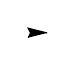
\begin{tikzpicture}[scale=\myscale,rotate=-90]
%	\useasboundingbox (0,-.4) rectangle (0,.4);
	\filldraw (0,.4) -- (-.2,-.4) -- (0,-.3) -- (.2,-.4);
	\end{tikzpicture}
}};

%Arrow to represent Current
\node[label=above:$i_6$] at (11,0) 
{{
\begin{tikzpicture}[scale=\myscale,rotate=90]
%	\useasboundingbox (0,-.4) rectangle (0,.4);
	\filldraw (0,.4) -- (-.2,-.4) -- (0,-.3) -- (.2,-.4);
	\end{tikzpicture}
}};








%Node
\node at (6,6) 
{{\begin{tikzpicture}[scale=\myscale,rotate=-90]
%	\useasboundingbox (0,-.4) rectangle (0,.4);
	\filldraw (0,0) circle (.15cm);
	\end{tikzpicture}
}};

%Node
\node at (6,0) 
{{\begin{tikzpicture}[scale=\myscale,rotate=-90]
%	\useasboundingbox (0,-.4) rectangle (0,.4);
	\filldraw (0,0) circle (.15cm);
	\end{tikzpicture}
}};

%Node
\node at (12,0) 
{{\begin{tikzpicture}[scale=\myscale,rotate=-90]
%	\useasboundingbox (0,-.4) rectangle (0,.4);
	\filldraw (0,0) circle (.15cm);
	\end{tikzpicture}
}};

%Node
\node at (12,6) 
{{\begin{tikzpicture}[scale=\myscale,rotate=-90]
%	\useasboundingbox (0,-.4) rectangle (0,.4);
	\filldraw (0,0) circle (.15cm);
	\end{tikzpicture}
}};

\end{tikzpicture}

\\
Two Loop System & Three Loop System
\end{tabular}\end{center}
\caption{Electrical Circuit Diagrams.}
\label{ecir}\end{figure}
In this diagram, wires meet at nodes (illustrated with a dot).  
Batteries and voltage sources (represented by 
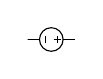
\begin{tikzpicture}[scale=.15,rotate=-90]
%	\useasboundingbox (-.5,-3) rectangle (.5,3);
	\clip (-1,-2) rectangle (1,2);
	\draw (0,0) circle (1cm);
	\draw (.3,.5) -- (-.3,.5);
	\draw (0,.2) -- (0,.8);
	\draw (.3,-.5) -- (-.3,-.5);
	\draw (0,1) -- (0,3);
	\draw (0,-1) -- (0,-3);
\end{tikzpicture}
or other symbols)
supply a voltage of $E$ volts.  At each node the current may change, so the arrows and letters $i$ represent the different currents in the electrical system. The electrical current on each wire may or may not follow the arrows drawn (a negative current means that the current flows opposite the arrow). Resistors are depicted with the symbol 	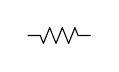
\begin{tikzpicture}[scale=.2,rotate=90]
%	\useasboundingbox (0,-3) rectangle (0,3);
	\clip (-.5,-2) rectangle (.5,2);
	\draw (0,-3) -- ++(0,1.8) -- ++(.5,.2) 
		-- ++(-1,.4) -- ++(1,.4)
		-- ++(-1,.4) -- ++(1,.4)
		-- ++(-1,.4) -- ++(.5,.2)
		-- ++(0,1.8) ;
	\end{tikzpicture}
, and the letter $R$ represents the ohms. 

Kirchoff discovered two laws. They both help us find current in a system, provided we know the voltage of any batteries, and the resistance of any resistors. 
\begin{enumerate}
	\item Kirchoff's current law states that at every node, the current flowing in equals the current flowing out (at nodes, current in = current out). 
	\item Kirchoff's voltage law states that on any loop in the system, the directed sum of voltages supplied equals the directed sum of voltage drops (in loops, voltage in = voltage out). 
\end{enumerate}

Let's use Kirchoff's laws to generate a system of equations for the two loop system. 
\begin{problem}
 Set up the two loop problem in general. Then give them some coefficients and have them solve.
%I'll need this at some point.
$$
\begin{array}{rl}
i_1-i_2-i_3&=0\\
R_1i_1+R_2i_2&=E\\
-R_2 i_2 +R_3i_3&=0
\end{array}
$$
\end{problem}

\begin{problem}
 Set up the three loop problem in general, and then solve with some specific coefficients.
\end{problem}




\subsection{Stoichiometry}
Chemical reaction stoichiometry is the study balancing chemical equations. A chemical reaction will often transform reactants into by-products. The by products are generally different compounds, together with either an increase or decrease in heat. One key rule in stoichiometry is that a chemical process neither creates nor destroys matter, rather it only changes the way the matter is organized. For simple reactions (with no radioactive decay), this conservation law forces the number of atoms entering a reaction to be the same as the number leaving. The next problem asks you to use this conservation law to create a balanced chemical reaction equation. 
\begin{problem}
 The chemical compound hydrocarbon dodecane ($C_{12}H_{26}$) is used as a jet fuel surrogate (see Wikipedia for more info).  This compound reacts with oxygen $(0_2)$, and the chemical reaction produces carbon dioxide ($CO_2$), water ($H_2 0$), and heat.  Suppose we expose some dodecane to oxygen, and that a chemical reaction occurs in which the dodecane is completely converted to carbon dioxide and water.  
 Conservation requires that the number of atoms ($H$, $C$, and $0$) at the beginning of the chemical reaction must be the exact same as the number at the end. 
 We could write the chemical reaction in terms of molecules as
 $$x_1 C_{12}H_{26} +x_2 O_2 = x_3 CO_2+ x_4 H_2O\quad \text{or} \quad x_1 C_{12}H_{26} -x_2 O_2 = x_3 CO_2- x_4 H_2O=0, $$
 where $x_1$ molecules of dodecane and $x_2$ molecules of oxygen were converted to $x_3$ units of carbon dioxide and $x_4$ units of oxygen.  
 If we look at each atom (carbon, hydrogen, and oxygen) individually, we obtain three equations to relate the variables $x_1, x_2, x_3, x_4$.  The carbon equation is simply
 $$x_1(12) + x_2(0) = x_3(1)+x_4(0) \quad \text{or}\quad x_1(12) + x_2(0) - x_3(1)-x_4(0)=0.$$  
 Your job follows:
\begin{enumerate}
 \item Write the other two conservation equations (for hydrogen and oxygen). 
 \item Solve the corresponding system of equations by row reduction.  As there are only 3 equations with 4 unknowns, you should obtain infinitely many solutions. Write each variable in terms of the free variable.  
 \item If about 10,000 molecules of water are present at the end of the reaction, about how many molecules of dodecane were burned? 
\end{enumerate}
\end{problem}


\section{Cramer's Rule}
Gabriel Cramer developed a way to solve linear systems of equations by using determinants. For small systems, the solution is extremely fast.  However, for large systems, the method looses it's power because of the complexity of computing determinants.  Also, when the coefficients in the system are variables, Cramer's rule provides an extremely fast algorithm for computing determinants. I'll remind you occasionally throughout the problem set to apply Cramer's rule when the problem involves variable coefficients.
\begin{theorem}[Cramer's Rule]\label{Cramer's Rule}
 Consider the linear system given by $A\vec x = \vec b$, where 
$A=\begin{bmatrix}\vec v_1 &\vec v_2 &\cdots \vec v_n \end{bmatrix}$
is an $n$ by $n$ matrix whose determinant is not zero.  Let $D=|A|$. For each $i$, replace vector $\vec v_i$ with $\vec b$, and then let $D_i$ be the determinant of the corresponding matrix. The solution to the linear system is then 
$$x_1 = \frac{D_1}{D},\quad x_2 = \frac{D_2}{D},\quad \cdots \quad x_n = \frac{D_n}{D}.$$

For the 2 by 2 system
$$
\begin{bmatrix}\nvec{a_{11}\\a_{21}}&\nvec{a_{12}\\a_{22}} \end{bmatrix}
\begin{bmatrix}\nvec{x_{1}\\x_{2}} \end{bmatrix}
=
\begin{bmatrix}\nvec{b_{1}\\b_{2}} \end{bmatrix},
$$
Cramer's rule states the solution is (provided $|A|\neq 0$) 
$$
x_1 = \frac{D_1}{D}=\frac{\begin{vmatrix}\nvec{b_1\\b_2}&\nvec{a_{12}\\a_{22}} \end{vmatrix}}{\begin{vmatrix}\nvec{a_{11}\\a_{21}}&\nvec{a_{12}\\a_{22}} \end{vmatrix}},
\quad 
x_2 = \frac{D_2}{D}=\frac{\begin{vmatrix}\nvec{a_{11}\\a_{21}}&\nvec{b_1\\b_2}\end{vmatrix}}{\begin{vmatrix}\nvec{a_{11}\\a_{21}}&\nvec{a_{12}\\a_{22}} \end{vmatrix}}
.$$
% For the 3 by 3 system
% $$
% \begin{bmatrix}\nvec{a_{11}\\a_{21}\\a_{31}}&\nvec{a_{12}\\a_{22}\\a_{32}}&\nvec{a_{13}\\a_{23}\\a_{33}} \end{bmatrix}
% \begin{bmatrix}\nvec{x_{1}\\x_{2}\\x_3} \end{bmatrix}
% =
% \begin{bmatrix}\nvec{b_{1}\\b_{2}\\b_3} \end{bmatrix},
% $$
% Cramer's rule states the solution is (provided $|A|\neq 0$) 
% $$
% x_1 = \frac{D_1}{D}=\begin{vmatrix}\nvec{b_1\\b_2\\b_3}&\nvec{a_{12}\\a_{22}\\a_{32}}&\nvec{a_{13}\\a_{23}\\a_{33}} \end{vmatrix},
% \quad 
% x_2 = \frac{D_2}{D}=\begin{vmatrix}\nvec{a_{11}\\a_{21}\\a_{31}}&\nvec{b_1\\b_2\\b_3}&\nvec{a_{13}\\a_{23}\\a_{33}}\end{vmatrix}
% \quad 
% x_3 = \frac{D_3}{D}=\begin{vmatrix}\nvec{a_{11}\\a_{21}\\a_{31}}&\nvec{a_{12}\\a_{22}\\a_{32}}&\nvec{b_1\\b_2\\b_3}\end{vmatrix}
% .$$

\end{theorem}


\begin{problem}
 Consider the system of equations $x+2y=3, 4x+5y=6$. Solve this system in 2 different ways.
\begin{enumerate}
 \item Use Cramer's rule to solve the system. You just need to compute three 2 by 2 determinants.
 \item Use row reduction to solve the system. Show the steps in class. 
\end{enumerate}
\end{problem}

In the next problem, you'll provide a proof of Cramer's rule in 2D. Your proof will contain the key idea needed to prove the theorem in all dimensions. The key idea is to connect determinants to areas of parallelograms.  
\begin{problem}[Proof of Cramer's Rule]
Let $\vec v_1 = (2,-2)$ and $\vec v_2 = (1,2)$. Let $x_1=-3$ and $x_2 = -2$, which means that $\vec b = x_1\vec v_1+x_2\vec v_2=(-8,2)$. In the picture below, the solid red vector is $\vec v_1$, the solid blue vector is $\vec v_2$, and the solid black vector is $\vec b$. Use the picture below, to answer the following questions.

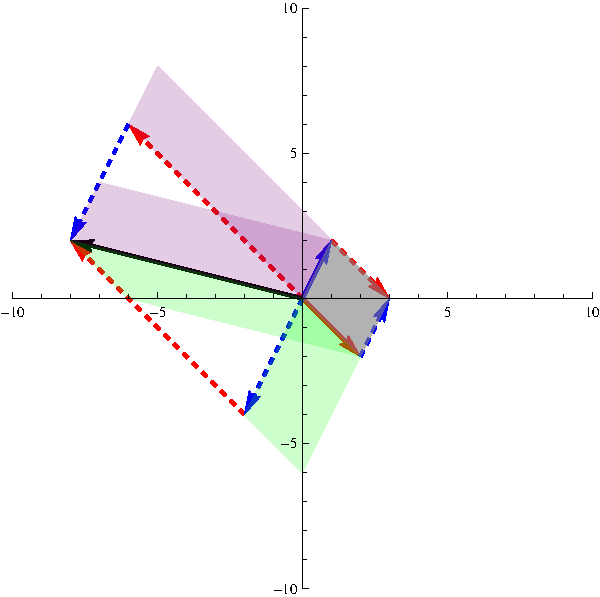
\includegraphics{cramers-visual}

\noindent[Hint: Each question can be answered by thinking about determinants as areas.]
\begin{enumerate}
 \item Explain why $x_1\begin{vmatrix}\vec{v_1}&\vec v_2\end{vmatrix}=\begin{vmatrix}x_1\vec{v_1}&\vec v_2\end{vmatrix}$.  Then explain why $\begin{vmatrix}x_1\vec{v_1}&\vec v_2\end{vmatrix} = \begin{vmatrix}\vec{b_1}&\vec v_2\end{vmatrix}$.  Finally, solve for $x_1$ to show $$x_1 = \frac{D_1}{D}=\frac{\begin{vmatrix}\nvec{b_1\\b_2}&\nvec{a_{12}\\a_{22}} \end{vmatrix}}{\begin{vmatrix}\nvec{a_{11}\\a_{21}}&\nvec{a_{12}\\a_{22}} \end{vmatrix}}.$$
 \item In a similar fashion, obtain a formula for $x_2$. 
\end{enumerate}
\end{problem}

\begin{problem}
 In problem .... we obtained the matrix equation ....  Use Cramer's rule to obtain the solutions to this system of equations. 
\end{problem}


Cramer's rule is most useful when the coefficients in the linear system are variables, rather than numbers.  
Let's apply our knowledge to study the arms race (the building of armies - tanks, bombs, soldiers, etc. - between two countries).  Consider two countries, country $A$ and country $B$. As country $B$ builds up their military, country $A$ looks on and says ``Hmm, we better build up our military.''  Similarly, as country $A$ builds up their military, country $B$ looks and says, ``Hmm, we better build up our military.''  If country $A$ has a grudge against country $B$, they will probably build up their military regardless of what country $B$ does.  Similarly, any past grievances and grudges that country $B$ has against country $A$ will increase the rate at which country $B$ builds up their military. Building up a military costs money, so hopefully both countries have economic limitations that restrict the growth of their military. The real question behind the arms race is, ``Will the two countries eventually decide they are spending enough on their military, or will their spending continue to grow without bound.''

 We now develop a system of differential equations that describes the above.  The key principle is a general law of conservation:
\begin{quote}
 The change in a quantity equals the flow in of the quantity minus the flow out of the quantity, or more simply 
$$\text{Change = (Flow in) - (Flow out)}$$
$$\text{Change = (Increase) - (Decrease)}$$
\end{quote}
\begin{itemize}
\item Let $x$ represent the dollar amount per year that country $A$ spends on arms. Let $y$ represent the dollar amount per year that country $B$ spends on arms.  
\item When $y$ is large, country $A$ will respond by increasing their spending.  
We'll assume this change is proportional to $y$, so we see that $x$ increases by an amount $ay$. 
 Similarly, when $x$ is large, country $B$ responds by increasing their spending. Let's assume that $y$ increases by an amount $mx$.
\item The economy of each country tries to slow down the growth rate.  The more money country $A$ spends, the larger the effect of the economy.  We'll assume that $x$ decreases by an amount $bx$.  Similarly, we'll assume $y$ decrease by an amount $ny$.
\item If the countries hold grudges against each other for past grievances, then they are inclined to increase their spending regardless of economic factors and the growth of the other country's army.  Let $c$ represent the amount that country $A$ will increase their spending by, and let $p$ represent the amount that country $B$ will increase their spending by. These values might be zero (for example the US and Canada do not hold such grudges), but might not be zero at all (as was the cases during the cold war, between the US and USSR).
\end{itemize}

\begin{problem}
Read the arms race information above, and then answer the following questions.
\begin{enumerate}
 \item There are three things causing $x$ to change. The flow in (parts causing an increase) are $ay$ and $c$, the response to the other country, and any grudges.  The flow out (parts causing a decrease) is only $bx$, the economic restriction.  We can write this as a differential equation $$\frac{dx}{dt} = ay-bx+c.$$ Obtain a similar equation for $\dfrac{dy}{dt}$ (using the coefficients $m$, $n$, and $p$). Then write your system of ODEs in the form 
$$
\begin{bmatrix}x'\\y'\end{bmatrix}
=
\begin{bmatrix}b&-a\\?&?\end{bmatrix}
\begin{bmatrix}x\\y\end{bmatrix}
+
\begin{bmatrix}c\\?\end{bmatrix}.
$$ 
 \item An equilibrium solution to the system of differential equations above is a solution that remains stable. At equilibrium, there should not be any future change in $x$ nor $y$, so we should have $dx/dt=0$ and $dy/dt=0$. Find the equilibrium solution for the arms race problem. [Cramer's rule should make this really fast.]
 \item Find the eigenvalues of the square matrix from part 1. What conditions must be met so that both eigenvalues are negative? In class, we'll pick some positive values for $a,b,c,m,n,p$ that satisfy the conditions you tell us, and then graph the vector field $\frac{d \vec x}{dt} = A\vec x+\vec p$, along with some solution curves.  
\end{enumerate}
\end{problem}


\section{Curve Fitting}
\subsection{Interpolating Polynomials}
Through any two points (with different $x$ values) there is a unique line of the form $y=mx+b$. If you know two points, then you can use them to find the values $m$ and $b$.  Through any 3 points (with different $x$ values) there is a unique parabola of the form $y=ax^2+bx+c$, and you can use the 3 points to find the values $a,b,c$.  As you increase the number of points, there is still a unique polynomial (called an interpolating polynomial) with degree one less than the number of points, and you can use the points to find the coefficients of the polynomial. In this section we will find interpolating polynomials, and show how the solution requires solving a linear system.

To organize our work, let's first standardize the notation.  Rather than writing $y=mx+b$, let's write $y=a_0+a_1 x$ (where $a_0=b$ and $a_1=m$). For a parabola, let's write $\ds y=a_0 + a_1 x+ a_2 x^2 = \sum_{k=0}^{2} a_k x^k$. We can now write any polynomial in the form $$\ds y = a_0 + a_1 x+ \cdots + a_n x^n = \sum_{k=0}^n a_k x^k.$$ By standardizing the coefficients, we can use summation notation to express any degree polynomial by changing the $n$ on the top of the summation sign. 

\begin{problem}
 Answer the following by row reducing an appropriate matrix. Please show us the steps in your row reduction. [Hint: Each point produces an equation.]
\begin{enumerate}
 \item Find the intercept $a_0$ and slope $a_1$ of a line $y = a_0+a_1 x$ that passes through the points $(1,2)$ and $(3,5)$. [We could have use $m$ and $b$, but I chose to use $a_0$ and $a_1$ so you can see how this generalize quickly to all dimensions.]
 \item Find the coefficients $a_0$, $a_1$, and $a_2$ of a parabola $y = a_0+a_1 x^1+a_2x^2$ that passes through the points $(0, 1)$,  $(2, 3)$, and  $(−1, 4)$. [Hint: The second point produces the equation $3=a_0+a_1(2)+a_2(2)^2$.]
\end{enumerate}
\end{problem}

\begin{problem}
 Give an equation of a cubic polynomial $y = a_0+a_1x^1+a_2x^2+a_3x^3$ that passes through the four points $(0, 1)$, $(1, 3)$, $(−1, 4)$, and $(2, 4)$. Show us the steps in your row reduction. [Hint: Each point produces an equation.  You should have a linear system with 4 equations and 4 unknowns.]
\end{problem}


\begin{problem}
Solve the following. [Hint: Because the problem involves variable points, Cramer's rule will be much faster than row reduction.]
\begin{enumerate}
 \item Find the intercept $a_0$ and slope $a_1$ of a line $y = a_0+a_1 x$ that passes through the points $(x_1,y_1)$ and $(x_2,y_2)$. 
 \item Find the coefficients $a_0$, $a_1$, and $a_2$ of a parabola $y = a_0+a_1 x^1+a_2x^2$ that passes through the points $(x_1, y_1)$,  $(x_2, y_2)$, and  $(x_3, y_3)$.
\end{enumerate}
Under what conditions will your solutions above not be valid?
\end{problem}

If we collect 2 data points, then we can usually find an equation of a line that passes through them.  If we collect 3 data points, we can usually find an equation of a parabola passing through them.  Continuing in this fashion, if we collect $n+1$ data points, then we can usually find an equation of a polynomial of degree $n$ that passes through them.
\begin{problem}
Suppose that we collect the 6 data points $(1,1)$, $(2,3)$, $(-1,2)$, $(0,-1)$, $(-2,0)$, $(3,1)$. We would like to find a polynomial that passes through all 6 points. State the degree $n$ of this polynomial. Then find the coefficients $a_0, a_1, \ldots, a_n$ of this polynomial.  Please use technology to do your row reduction.  When you present in class, show us the matrix you entered into a computer, and then show us the reduced row echelon form together with the polynomial.
\end{problem}

\subsection{Least Squares Regression}

Interpolating polynomials give a polynomial which passes through every point
listed. While they pass through every point in a set of data, the more points
the polynomial must pass through, the more the polynomial may have to make
large oscillations in order to pass through each point. Sometimes all we want is a simple line or
parabola that passes near the points and gives a good approximation
of a trend in the data. When I needed to purchase a minivan for my expanding
family, I gathered mileage and price data for about 40 cars from the internet. I
plotted this data and discovered an almost linear downward trend (as mileage
increased, the price dropped). Using this data I was able to create a line to
predict the price of a car. I then used this data to talk the dealer into dropping
the price of their car by over \$1000. 
Finding an equation of this line, called
the least squares regression line, is the content of this section. In other words,
if you have 3 or more points, how do you find a line that is ”closest” to passing
through these points? The least squares regression line is used to find trends in
many branches of science, in addition to haggling for lower prices when buying
a car. Statistics builds upon this idea to provide powerful tools for predicting
the future.

\begin{problem}
Consider the three points $(2,4)$, $(0,1)$, and $(3,5)$. We wish to find a line $y=  a_0+a_1 x$ that fits this data.  
\begin{enumerate}
 \item What 3 equations do the points and line give.  Write the linear system as a matrix equation by filling in $A$ and $\vec b$ below:
 $$A\vec x=\vec b\quad\quad\text{or}\quad \quad\begin{bmatrix}1&2\\ ? &? \\ ?&? \end{bmatrix}\begin{bmatrix}a_0\\a_1\end{bmatrix}=\begin{bmatrix}4\\ ? \\ ? \end{bmatrix}.$$
 The first equation $4=a_0+a_1(2)$ is already on the first row.
 \item Row reduce the corresponding augmented matrix to show that this system has no solution. The problem is that we have more equations than we do unknowns. The system is overdetermined. 
 \item If we multiply both sides of the equation $A\vec x = \vec b$ by a 2 by 3 matrix $C$, then the product $CA$ will be a 2 by 2 matrix. We could then solve the system $CA\vec x = Cb$, as it would then have 2 equations and 2 unknowns. 

The only 2 by 3 matrix in the problem is the transpose of $A$.  So compute $A^TA$ and $A^T\vec b$.  Then solve the system $(A^T A)\vec x = A^T \vec b$. 
\end{enumerate}

\end{problem}

The previous problem suggests the following theorem.  One proof of this theorem involves projecting $\vec b$ onto the plane spanned by the columns of $A$. This proof leads to the ideas behind inner product spaces, the Graham Schmidt orthogonalization process, and more, something you would study near the end of math 341 (Linear Algebra).

\begin{theorem}[Least Squares Regression]
When we collect $n$ data points and notice the points follow a linear trend, the coefficients of the least square regression line $y=a_0+a_1x$ are the solutions to the equation $A^T A\vec x = A^T\vec b$, where we have $$
\vec x =
\begin{bmatrix}
a_0\\
a_1
\end{bmatrix}
,
A = \begin{bmatrix}
1&x_1\\
1&x_2\\ 
\vdots&\vdots\\
1&x_n
\end{bmatrix}
,
\vec b =
\begin{bmatrix}
y_1\\
y_2\\ 
\vdots\\
y_n
\end{bmatrix}
,\text{ and }
A = \begin{bmatrix}
1&1&\cdots&1\\
x_1&x_2&\cdots x_n
\end{bmatrix}
.$$
\end{theorem}

\begin{problem}\label{getting the least square regression coefficients using the transpose}
 Suppose you collect the $n$ data points $(x_1,y_1)$, $(x_2,y_2)$, $\ldots$, $(x_n,y_n)$, and you wish to find the least squares regression line $y=a_0+a_1x$. Set up the matrices $A$, $\vec x$, $\vec b$, and $A^T$. Multiply together $A^TA$ and $A^T\vec b$ (your result should involve sums of the form $\sum x_i$, $\sum y_i$, $\sum x_iy_i$, and $\sum x_i^2$). Then solve the equation $A^TA\vec x = A^T\vec b$ and state the coefficients $a_0$ and $a_1$. leas[Hint: Since the system involves variable coefficients, try using Cramer's rule. It will kick out the solution almost instantly.]
\end{problem}


The key to solving the overdetermined system $A\vec x=\vec b$ is to multiply each side on the left by a matrix $C$, so that the produce $CA$ is a square matrix. We then solve $CA\vec x = C\vec b$. The least square regression model comes by letting $C=A^T$.  We obtain alternate data fitting models by using a matrix other than $A^T$ (though this is a topic for another course).  The next problem has you find the best fitting parabola, using the least square regression model.
\begin{problem}
 Consider the 5 points $(-2,3)$, $(-1,1)$, $(0,-1)$, $(1,2)$, $(2,4)$, and . We would like to find an equation of a parabola $y = a_0 +a_1 x+ a_2x^2$ that approximates the trend in the data, using the least square regression model.  
\begin{enumerate}
 \item The 5 data points produce 5 equations in the three unknowns $a_0$, $a_1$, $a_2$. Write the linear system as a matrix equation by filling in $A$ and $\vec b$ below:
 $$A\vec x=\vec b\quad\quad\text{or}\quad \quad\begin{bmatrix}1&-2&4\\ ? &?&? \\ ?&?&?\\ ?&?&?\\ ?&?&? \end{bmatrix}\begin{bmatrix}a_0\\a_1\\a_2\end{bmatrix}=\begin{bmatrix}3\\ ? \\ ? \\ ? \\ ? \end{bmatrix}.$$
 \item Multiply both sides of the equation $A\vec x = \vec b$ by an appropriate 3 by 5 matrix $C$. Then solve the system $(C A)\vec x = C \vec b$. Feel free to use software to obtain your answer.  In class, just show us $CA$, $C\vec b$, and the rref of $\begin{bmatrix}CA&C\vec b\end{bmatrix}$.
 \item Plot the 5 data points and the parabola you found.
\end{enumerate}

\end{problem}




The next problem has the exact same solution as Problem \ref{getting the least square regression coefficients using the transpose}, but does not require you to use a matrix transpose, nor matrix multiplication. Instead, it focuses on setting partial derivative equal to zero, which is the first step in locating minimums. You then just have to solve a system of linear equations. 
\begin{problem}
 Suppose you collect the $n$ data points $(x_1,y_1)$, $(x_2,y_2)$, $\ldots$, $(x_n,y_n)$, and you wish to find the least squares regression line $y=a_0+a_1x$. 
 Each point $(x_i,y_i)$ produces an error $y-y_i = (a_0+a_1x_i)-y_i$. The least squares regression line is the line that minimized the sum of the squares of these errors, which means we need to minimize $$f(a_0,a_1) = \sum_{i=1}^n \left((a_0+a_1x_i)-y_i\right)^2.$$
\begin{enumerate}
 \item Compute $\dfrac{\partial f}{\partial a_0}$ and $\dfrac{\partial f}{\partial a_1}$. 
 \item Since we seek the minimum of $f$, solve the system  $\dfrac{\partial f}{\partial a_0}=0$ and $\dfrac{\partial f}{\partial a_1}=0$ for $a_0$ and $a_1$.  
\end{enumerate}
[Hint: Once you get each equation written in the form $(?)a_0 +(?)a_1 = ?$, use Cramer's rule to kick out the answer almost instantly.]
\end{problem}




\section{Vector Spaces and Linear Transformations}
Remind them of the idea about coordinate transformation from 215.  Polar coordinates is an example of such a transformation.  Now introduce them to linear transformations. Have them make connections about area, eigenvalues, and eigenvectors.

\begin{problem}
 Give them a linear transformation.  Have them compute the eigenvalues, eigenvectors, and determinant.  Then have them draw the image of an object, and determine it's area.  (How do connect eigenvalues --- have to think of the best problem).
\end{problem}

\begin{problem}
 Give them a before/after image.  Have them write down a linear transformation that would accomplish the transforming.  Stay in 2D to 2D.
\end{problem}

\begin{problem}
Jump to a 3D to 3D transformation.  Give them two different ones.  Have them determine volume in the new space.  Have one of them have dependent columns.  Ask them what the span is.
\end{problem}
 
\begin{problem}
 I need a problem that introduces the concept of rank and nullity of a linear transformation.  What is the dimension of the image space.  What is the dimension of the space that gets sent to zero. This will be the problem that introduces them to the kernel of a linear transformation.
\end{problem}

Define carefully a linear transformation.  Loosely define vector spaces.

\begin{problem}
 Is the derivative a linear transformation? Is an integral a linear transformation?  Is the Laplace Transform a linear transformation?
\end{problem}

\begin{problem}
 Have them solve a simple first order ODE, but make them use the language ``What is the kernel of this linear transformation?'' This should cement the language we'll use later one.  
\end{problem}























\end{document}



































\section{Partial Fraction Decompositions}
A partial fraction decomposition is a method of breaking a complex rational function up into the sum of smaller simpler functions to work with. We will be using partial fraction decompositions to rapidly solve differential equations throughout the semester (using Laplace transforms).  For now, we will start by gaining practice with partial fraction decompositions by integrating rational functions. To illustrate their value, let's start with an example.

\begin{example}
Let's find the integral of the function $\ds f(x)= {\frac {2x+1}{ \left( x-2 \right)  \left( x-3 \right) }}$. The denominator is the product of two linear functions. Is it possible to break up the function into two simpler functions, namely can we write 
$${\frac {2\,x+1}{ \left( x-2 \right)  \left( x-3 \right) }}={\frac {A}{
x-2}}+{\frac {B}{x-3}}$$
for unknown constants $A$ and $B$? If we multiply both sides by the original denominator, we obtain (cancel the common factors)
$$2x+1 = A(x-3)+B(x-2).$$
Now expand the right hand side and collect the terms which have the same powers of $x$, 
$$2x+1 = (A+B)x+(-3A-2B).$$
Both sides of the equation above represent lines. In order for the two lines to be the same line, they must have the same slope and intercept.  This means we can create an equation for each power of $x$ by equating the coefficients on both sides of the equation.  This gives us the two equations
$$2=A+B \quad \quad 1=-3A-2B.$$
This is a linear system and Gaussian elimination or Cramer's rule will solve it:
$$
\begin{bmatrix}[cc|c]
1&1&2\\
-3&-2&1
\end{bmatrix}
\xrightarrow{\text{rref}}
\begin{bmatrix}[cc|c]
1&0&-5\\
0&1&7
\end{bmatrix}
$$
The solution is $A=-5,B=7$ and so $\ds{\frac {2\,x+1}{ \left( x-2 \right)  \left( x-3 \right) }}={\frac {-5}{
x-2}}+{\frac {7}{x-3}}$. Finish by integrating each term separately to obtain 
$$\int{\frac {2\,x+1}{ \left( x-2 \right)  \left( x-3 \right) }}dx 
= \int {\frac {-5}{x-2}} dx +\int{\frac {7}{x-3}}dx
= {-5}\ln|{x-2}|+7\ln|{x-3}|.
$$
\end{example}

\subsection{Finding the correct form}
The general process for finding a partial fraction decomposition requires that you start with an appropriate guess for the final form, multiply both sides by the original denominator, collect like powers of $x$ on both sides, and then solve the corresponding linear system. How do you pick an appropriate guess to begin with?  Before giving the full idea, let's look at a simple example involving only integers and fractions, before generalizing to polynomials.

 The fraction $\frac{1}{6} = \frac{1}{2\cdot 3}$ can be written as a sum of two fractions with simpler denominators as $\frac16=\frac12-\frac13$. The prime factors of 6 are 2 and 3, so we decompose the more complicated fraction $\frac16$ into two simpler fractions whose denominators are the factors of 6. The fraction $\frac{5}{9} = \frac{5}{3\cdot 3}$ has a repeated factor of $3$ in the denominator, and can be written as $\frac{5}{9} = \frac{1}{3}+\frac{2}{3^2}$. This simplifies the numerators so that they are all less than the denominator. Improper fractions (a larger numerator than denominator) are written in proper form and then we decompose the remainder, as in $\frac{14}{9}=1+\frac59$ which then becomes $1+\frac13+\frac29$ after decomposing the fraction.
 
In a similar manner, the way we decompose a rational function depends on the factors of the denominator.  If the degree of th numerator is larger than the denominator, you start by performing long division to force the degree of the numerator to be smaller than the denominator.  Then find the factors of the denominator.  The appropriate guess for your partial fraction decomposition 
\begin{enumerate}
	\item Include a term for every factor of the denominator.
	\item The numerator of each term is one degree less than the degree of the factor (so constants go above linear factors, and linear terms go above quadratic factors).
	\item If a factor is a repeated factor, then it should be included each time, with an increasing power in the denominator.
\end{enumerate}
A proper partial fraction decomposition form will have the same number of unknowns as the degree of the denominator.
 
\begin{example} Let's illustrate the ideas above by picking the appropriate partial fraction decomposition form for the following rational functions:
\begin{enumerate}
	\item $\dfrac{2x+3}{x^2-1}$
	\item $\dfrac{x+1}{x^3+x}$
	\item $\dfrac{3x+2}{x^2+2x+1}$
	\item $\dfrac{x^4+2x-1}{x(x-1)^3(x^2+4x+5)(x^2+1)^2}$
\end{enumerate}

For the first, the denominator factors as two linear terms $(x-1)(x+1)$. Since both of these are linear, we place constants above each one to obtain $$\frac{2x+3}{x^2-1} = \frac{A}{x-1}+\frac{B}{x+1}.$$ There are two unknowns, which matches the degree of the denominator.

The denominator of the second factors as $x(x^2+1)$.  The quadratic term does not factor any more over real number (its zeros are $\pm\sqrt{-1}$), so we place a linear guess above it.  This gives
$$\frac{x+1}{x^3+x} = \frac{A}{x}+\frac{Bx+C}{x^2+1}.$$

On the third, the denominator factors as $(x+1)^2$.  Because this is a repeated factor, it get's included twice, but each time we include it we increase the power on the denominator.  Because the factor is linear, we place a constant above each term. This gives $$\frac{3x+2}{x^2+2x+1} = \frac{A}{x+1}+\frac{B}{(x+1)^2}.$$

On the last example, the denominator is already factored.  Each quadratic factor needs a linear term placed above it.  The form is 
\begin{align*}
\frac{x^4+2x-1}{x(x-1)^3(x^2+4x+5)(x^2+1)^2}
=&
\frac{A}{x}+
\frac{H}{x-1}+
\frac{I}{(x-1)^2}+
\frac{J}{(x-1)^3}\\
&+\frac{Bx+C}{x^2+4x+5}+
\frac{Dx+E}{x^2+1}+
\frac{Fx+G}{(x^2+1)^2}.
\end{align*}
Notice that there are 10 unknowns, which is the degree of the denominator.

\end{example}





\subsection{Integrating Rational Functions}
A rational function is the quotient of two polynomials, $r(x) = \frac{p(x)}{q(x)}$. If we can factor the denominator into products of linear and quadratic terms, then we can always integrate the rational function by performing a partial fraction decomposition and then integrating each term.  The three key integrals used to are $\int \frac{1}{x-a}dx = \ln|x-a|$, $\int \frac{1}{x^2+1}dx = \arctan x$, and $\int \frac{x}{x^2+1}dx = \frac{1}{2}\ln(x^2+1)$. You may have to complete the square and perform a $u$-substitution to reduce the integrals to one of these 3 key integrals.
  

\begin{example}
Let's compute $\int {\frac {-{x}^{2}+2\,x+5}{ \left( {x}^{2}+1 \right)  \left( x-3
 \right) }}dx$, using the form  
$${\frac {-{x}^{2}+2\,x+5}{ \left( {x}^{2}+1 \right)  \left( x-3
 \right) }}={\frac {Ax+B}{{x}^{2}+1}}+{\frac {C}{x-3}}.$$
In this case the denominator doesn't factor into a product of linear terms, so the quadratic term $x^2+1$ has a linear term $Ax+B$ in the numerator.  Multiplying both sides by the denominator and collecting powers of $x$ gives
$$-{x}^{2}+2\,x+5= \left( A+C \right) {x}^{2}+ \left( B-3\,A \right) x+(C-3\,B).$$
Equating the coefficients of $x$ on each side gives the three equations 
$$5=C-3B, 2=B-3A, -1=A+C$$
Rewriting in matrix form and reducing the matrix gives us
$$
\begin{bmatrix}[ccc|c] 
0&-3&1&5\\
-3&1&0&2\\
1&0&1&-1
\end {bmatrix}
\xrightarrow{\text{rref}}
\begin{bmatrix}[ccc|c]
1&0&0&-6/5\\
0&1&0&-8/5\\
0&0&1&1/5
\end {bmatrix} .
$$
We can now integrate using our solution to obtain 
\begin{align*}
\int {\frac {-{x}^{2}+2\,x+5}{ \left( {x}^{2}+1 \right)  \left( x-3\right) }}dx
&= \int {\frac{1}{5}\left(\frac {-6x-8}{{x}^{2}+1}\right)}+ \frac{1}{5}\left({\frac {1}{x-3}}\right)dx \\
&= -\frac{6}{5}\int \frac{x}{x^2+1}dx -\frac{8}{5}\int \frac{1}{x^2+1}dx +\frac{1}{5}\int{\frac {1}{x-3}}dx\\
&= -\frac{6}{10}\ln|{x^2+1}| -\frac{8}{5}\arctan x +\frac{1}{5}\ln|{x-3}|+C.
\end{align*}
\end{example}












